\documentclass[30pt,twocolumn,letterpaper]{article}
\usepackage{cvpr}
\usepackage{times}
\usepackage{booktabs}
\usepackage{epsfig}
\usepackage{graphicx}
\usepackage{amsmath}
\usepackage{amssymb}
\cvprfinalcopy
\def\cvprPaperID{****}
\def\httilde{\mbox{\tt\raisebox{-.5ex}{\symbol{126}}}}
\usepackage{graphicx}
\usepackage{indentfirst}
\setlength{\parindent}{2em}
\usepackage{cite}
\usepackage[colorlinks,linkcolor=red,anchorcolor=blue,citecolor=green,backref=page]{hyperref}
\author{Qilei Zhang\\\\
Jun 20 2018}
\title{Policy Distillation}
\begin{document}
\maketitle
\begin{abstract}
  Policies for complex visual tasks have been successfully learned with deep reinforcement learning, using an approach called deep Q-networks (DQN), but relatively large (task-specific) networks and extensive training are needed to achieve good performance.
\end{abstract}
\section{Introduction}
Recently, advances in deep reinforcement learning have shown that policies can be encoded through end-to-end learning from reward signals\cite{Gaminibandara1976Synthesis}, and that these pixel-to-action policies can deliver superhuman performance on many challenging tasks\cite{Kupferberg1968The}. \\
\begin{figure}[htbp]
\small
\centering
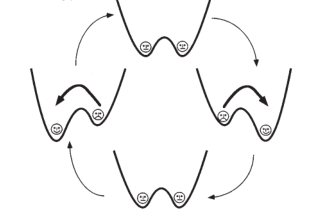
\includegraphics[width=20em]{000.png}
\caption{Example frames from two Atari games, with the Q-values output by DQN (top) and the distillation
targets after softmax (middle). For Pong, the two frames only differ by a few pixels yet the Q-values are
different. In the Space Invaders example, the input frames are very different yet the Q-values are very similar.
In both games the softmax sharpens the targets, making it easier for the student to learn.}
\label{fig:lable}
\end{figure}\\
\begin{equation}
\quad x'(t)=-V'(x)+A_0cos(wt+o)+u(t)
\end{equation}
\section{Previous Work}
This work is related to four different research areas: model compression using distillation, deep reinforcement learning\cite{Li1998Adaptive}, multi-task learning and imitation learning. The concept of model compression through training a student network using the outputs of a teacher network was first suggested by Bucila who proposed it as a means of compressing a large ensemble model into a single network\cite{Wozny2002Optimisation}.\\
\begin{figure}[htbp]
\small
\centering
\includegraphics[width=20em]{001.png}
\caption{: (a) Single-task data collection and policy distillation. The DQN agent periodically adds gameplay to
the replay memory while the student network is trained. (b) Multi-task data collection and policy distillation.
}
\label{fig:lable}
\end{figure}\\

\begin{table}
\begin{center}
\begin{tabular}{ccccc}
\toprule
         & DQN  &Dist-MSE&Dist-NLL&Dist-KL\\
\midrule
         &score &score   &score   &score\\
 Breakout&303.9 &102.9   &235.9   &287.8\\
 Freeway &25.8  &25.7    &26.2    &26.7\\
 Pong    &16.2  &15.3    &15.4    &16.3\\
 Qbret   &4589.8&5607.3  &6773.5  &7112.8\\
 \bottomrule
\end{tabular}
\end{center}
\caption{: Comparison of learning criteria used for policy distillation from DQN teachers to students with identical
network architectures: MSE (mean squared error), NLL (negative log likelihood), and KL (Kullback-Leibler
divergence). Best relative scores are outlined in bold}
\end{table}
\section{Approach}
Before describing policy distillation, we will first give a brief review of deep Q-learning, since DQN serves as both the baseline for performance comparisons as well as the teacher for the policy distillation. Note that the proposed method is not tied to DQN and can be applied to models trained using other RL algorithms. After the DQN summary, we will describe policy distillation for single and multiple tasks\cite{ZHANG2006A}.
{\small
\bibliographystyle{ieee}
\bibliography{1}
}
\end{document}
